% 页面设置
\documentclass[12pt, a4paper]{article} % 字号:12,纸张:A4
\usepackage[top=2.54cm, bottom=2.54cm, left=3.18cm,right=3.18cm]{geometry} % 页边距设置
% 字体设置
\usepackage[UTF8]{ctex}
\usepackage{fontspec} % 设置字体
%\setCJKmainfont{SimSun}[AutoFakeBold=true, BoldFont={SimHei}, ItalicFont={KaiTi}] % 正文字体
%\setCJKsansfont[AutoFakeBold=3]{KaiTi} % 无衬线字体
%\setCJKmonofont[AutoFakeBold=3]{SimHei} % 等宽字体
\setmainfont{Times New Roman} % 设置主字体为新罗马体
% 文本设置
\usepackage{enumerate} % 支持小标题编号
\linespread{1.5} % 行间距1.5倍
\usepackage{indentfirst}%首段缩进
\setlength{\parindent}{2em} % 首行缩进两字符
\usepackage[hidelinks]{hyperref} % 目录添加超链接
\usepackage{zhnumber} % 章节标题中文显示
\usepackage[cmyk]{xcolor} % 文字彩色显示
% 数学支持
\usepackage{amsmath} % 数学公式支持
\usepackage{amssymb} % 数学符号支持
\usepackage{bm} % 公式加粗
\usepackage{mathrsfs} % 花体字母
\usepackage{yhmath} % 更多的数学符号
% 图片设置
\usepackage{caption} % 插入图片标题
\usepackage{float} % 控制图片位置
\usepackage{subfigure} % 图片并排
\usepackage{booktabs} % 插入表格
% 表格设置
\usepackage{multirow} % 表格自动换行
\usepackage{bigstrut} % 表格间距
\usepackage{rotating} % 表格旋转
\usepackage{tabularx} % 表格宽度
\usepackage{colortbl} % 表格颜色
\usepackage{graphicx} % 表格自动宽度

\title{第二章 \ \ \ 模型评估与选择} % 文章标题
\author{Castor Ye} % 文章作者
\date{} % 文章时间

\begin{document} % 文档从这里开始。
\maketitle % 按照预定的模板把上面那些信息排好。
\newtheorem{definition}{定义}[section]
\newtheorem{theorem}{定理}[section]
\newtheorem{example}{例}[section]
\newtheorem{solution}{题解}
\newtheorem{algorithm}{算法}
\newtheorem{axiom}{公理}
\newtheorem{property}{性质}
\newtheorem{proposition}{命题}
\newtheorem{lemma}{引理}
\newtheorem{corollary}{推论}[section]
\newtheorem{remark}{注解}
\newtheorem{condition}{条件}
\newtheorem{conclusion}{结论}
\newtheorem{assumption}{假设}
\renewcommand{\figurename}{图} % 将图片序号改为图
\renewcommand{\tablename}{表} % 将表格序号改为表
%%%%%%%%%%%%%%%%%%%%%%%%%%%%%%%%%%%%%%%%%%%%%%%%%%%%%%%%%%%%%%%%%%%%%%%
% 文章内容从此开始
\section{经验误差与过拟合}

一般地,我们把学习器的实际预测输出与样本的真实输出之间的差异称为“误差”(error),学习器在训练集上的误差称为“训练误差”(training error)或“经验误差”(empirical error),在新样本上的误差称为“泛化误差”(generalization error)。

显然,我们希望得到的是在新样本上表现很好地学习器,即泛化误差小的学习器。因此我们应该从训练样本中尽可能学出适用于所有潜在样本的“普遍规律”。然而,当学习器把训练集学得“太好”的时候,即把一些训练样本的自身特点当成了普遍特征,这种情况在机器学习中称为“过拟合”(overfitting)。同时也有学习能力不足的时候,即训练集的基本特征都没有学习出来,我们称之为“欠拟合”(underfitting)。

可以得知:在过拟合问题中,训练误差十分小,但测试误差较大;在欠拟合问题中,训练误差和测试误差都比较大。目前,欠拟合问题比较容易克服,例如增加迭代次数等。但过拟合问题还没有十分好的解决方案,过拟合是机器学习面临的关键障碍。

\section{评估方法}

在现实任务重,我们往往有多种算法可供选择,那么我们应该选择哪一个算法才是最合适的呢?如上所述,我们希望得到的是泛化误差小的学习器,理想的解决方案是对模型的泛化误差进行评估,然后选择泛化误差最小的那个学习器。但是,泛化误差指的是模型在所有新样本上的适用能力,我们无法直接获得泛化误差。

因此,通常我们采用一个“测试集”来测试学习器对新样本的判别能力,然后以“测试集”上的“测试误差”作为“泛化误差”的近似。显然,我们选择的测试集应与训练集互斥。

可是,我们只有一个包含 $m$ 个样例的数据集 $D = \{(x_1, y_1), (x_2, y_2), \cdots, (x_m, y_m)\}$,既要训练,又要测试,怎么才能做到呢?我们可以通过对 $D$ 进行适当的处理,从中生成训练集 $S$ 和测试集 $T$,下面介绍几种常见的做法:

\subsection{留出法}

“留出法”(hold-out)直接将数据集 $D$ 划分为两个互斥的集合,其中一个集合作为训练集 $S$,另一个作为测试集 $T$,即 $D = S \cup T, S \cap T = \emptyset$。在 $S$ 上训练模型后,用 $T$ 来评估其测试误差,作为对泛化误差的估计。

由于划分的随机性,单词的留出法结果往往不够稳定,一般要采用若干次随机划分,重复实验取平均值的做法。

\subsection{交叉验证法}

“交叉验证法”(cross validation)先将数据集 $D$ 划分为 $k$ 个大小相似的互斥子集,即 $D = D_1 \cup D_2 \cdots \cup D_k, D_i \cap D_j = \emptyset$。每个自己 $D_i$ 都尽量保持数据分布的一致性,即从 $D$ 中通过分层采样得到。

交叉验证法的思想是:每次用 $k - 1$ 个子集的并集作为训练集,余下的那个子集作为测试集;这样就可以获得 $k$ 组不同训练集和测试集,即进行 $k$ 次训练和测试,最终返回 $k$ 次测试结果的均值。

交叉验证法也称“$k$ 折交叉验证”,$k$ 最常用的取值为 $10$,下图给出了 $10$ 折交叉验证的示意图:

\begin{figure}[H]
    \centering
    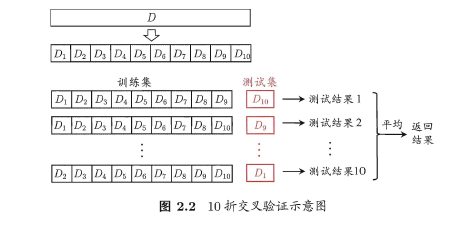
\includegraphics[width=0.7\textwidth]{../img/2-1-10折交叉验证.png}
    \caption{10 折交叉验证}
    \label{fig:10 折交叉验证}
\end{figure}

与留出法类似,将数据集 $D$ 划分为 $k$ 个子集的过程具有随机性,因此 $k$ 折交叉验证通常也要重复 $p$ 次,称为 $p$ 次 $k$ 折交叉验证。常见的是 $10$ 次 $10$ 折交叉验证。

\subsection{自助法}

我们希望评估的是用 $D$ 训练出的模型,但在留出法和交叉验证法中,由于保留了一部分样本用于测试,因此实际评估的模型所使用的训练集比 $D$ 小,这必然会引入一些因训练样本规模不同而导致的估计偏差。

“自助法”(bootstrapping)的基本思想是:给定包含 $m$ 个样本的数据集 $D$,我们对它进行采样产生数据集 $D ^\prime$,每次随机从 $D$ 中挑选一个样本,将其拷贝放入 $D ^\prime$,然后再将该样本放回初始数据集 $D$ 中,使得该样本在下次采样时仍有可能被采到。重复执行 $m$ 次,我们就得到了一个包含 $m$ 个样本的数据集 $D ^\prime$。可以得知,在 $m$ 次采样中始终不被采到的概率是:

\begin{equation}
    \lim_{m \to \infty} (1 - \frac{1}{m})^m = \frac{1}{e} \approx 0.368
\end{equation}

这样,通过自助采样,初始样本集 $D$ 中大约有 $36.8\%$ 的样本未出现在采样数据集 $D ^\prime$ 中。于是,我们可以将 $D ^\prime$ 作为训练集,$D - D^\prime$ 作为测试集。

自助法在数据集较小,难以有效划分训练集和测试集时很有用,但由于自助法产生的数据集(随机抽样)改变了初始数据集的分布,因此引入了估计偏差。在数据集足够时,留出法和交叉验证更加常用。

\subsection{调参与最终模型}

大多数学习算法都有些参数(parameter)需要设定,参数配置不同,学得模型的性能往往有显著区别。因此,在进行模型评估与选择时,除了要对适用的学习算法的选择,还需对算法参数进行设定,这就是通常所说的“参数调节”或简称“调参”(parameter tuning)。

\section{性能度量}

对学习器的泛化性能进行评估,不仅需要有效可行的实验估计方法,还需要有衡量模型泛化能力的评价标准,这就是性能度量(performance measure)。性能度量反映了任务需求,在对比不同模型的能力时,使用不同的性能度量往往会导致不同的评判结果;这意味着模型的“好坏”是相对的,什么样的模型是好的,不仅取决于算法和数据,还决定于任务需求。

在预测任务中,给定样例集 $D = \{(x_1, y_1), (x_2, y_2), \cdots, (x_m, y_m)\}$ 其中 $y_i$ 是示例 $x_i$ 的真实标记。要评估学习器  $f$ 的性能,就要把学习器预测结果 $f(x)$ 与真实标记 $f$ 进行比较。

回归任务最常用的性能度量是“均方误差”(mean squard error):
\begin{equation*}
    E(f; D) = \frac{1}{m} \sum_{i = 1}^{m} (f(x_i) - y_i)^2
\end{equation*}

更一般的,对于数据分布 $D$ 和概率密度函数 $p(\cdot)$,均方误差可以描述为:
\begin{equation*}
    E(f; D) = \int_{x \sim D} (f(x) - y)^2 p(x) dx
\end{equation*}

注意:
\begin{enumerate}[\hspace*{2em} i.]
    \item $(f; D)$ 为列向量,表示 $\displaystyle \left( {\begin{array}{*{20}{c}}
                      f \\
                      D
                  \end{array}} \right)$
\end{enumerate}

本节下面主要介绍分类任务中常用的性能度量。

\subsection{错误率与精度}

错误率是分类错的的样本数占样本总数的比例,精度则是分类正确的样本数占样本总数的比例。对样例集 $D$,分类错误率定义为:
\begin{equation*}
    E(f; D) = \frac{1}{m} \sum_{i = 1}^{m} \mathbb{I} (f(x_i) \ne y_i)
\end{equation*}

精度则定义为:
\begin{equation*}
    acc(f; D) = \frac{1}{m} \sum_{i = 1}^{m} \mathbb{I} (f(x_i) = y_i) = 1 - E(f; D)
\end{equation*}

更一般的,对于数据分布 $D$ 和概率密度函数 $p(\cdot)$,错误率和精度可分别描述为:
\begin{equation*}
    E(f; D) = \int_{x \sim D} \mathbb{I} (f(x) \ne y) p(x) dx
\end{equation*}
\begin{equation*}
    acc(f; D) = \int_{x \sim D} \mathbb{I} (f(x) = y) p(x) dx
\end{equation*}

注意:
\begin{enumerate}[\hspace*{2em} i.]
    \item $\mathbb{I} (\cdot)$ 为指示函数,在 $\cdot$ 为真和假时分别为 $1, 0$。
\end{enumerate}

\subsection{查准率、查全率与 F1}

对于二分类问题,可将样例根据其真实类别与学习器预测类别的组合划分为:真正例(true positive)、假正例(false positive)、真反例(true negative)、假反例(false negative)四种情形,令 $TP, FP, TN, FN$ 分别表示其对应的样例数,显然有 $TP + FP + TN + FN = $ 样例总数。

分类结果的“混淆矩阵”(confusion matrix)如下图所示:

\begin{figure}[H]
    \centering
    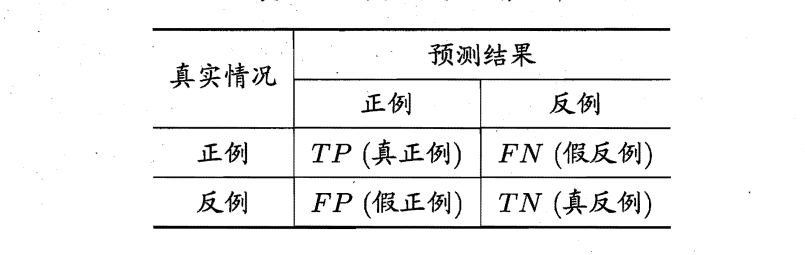
\includegraphics[width=0.8\textwidth]{../img/2-2-分类结果混淆矩阵.png}
    \caption{分类结果混淆矩阵}
    \label{fig:分类结果混淆矩阵}
\end{figure}

则,我们定义查准率 $P$ 和查全率 $R$ 为:
\begin{equation*}
    P = \frac{TP}{TP + FP}, R = \frac{TP}{TP + FN}
\end{equation*}

在很多情形下,我们可根据学习器的预测结果对样例进行排序,排在前面的是学习器认为“最可能”是正例的样本,排在最后的则是学习器认为“最不可能”是正例的样本。按此顺序逐个把样本作为正例进行预测,则每次可以计算出当前的查全率、查准率。以查准率为纵轴,查全率为横轴作图,就得到了查准率-查全率曲线,简称“$P-R$ 曲线”,显示该曲线的图称为“$P-R$ 图”。

\begin{figure}[H]
    \centering
    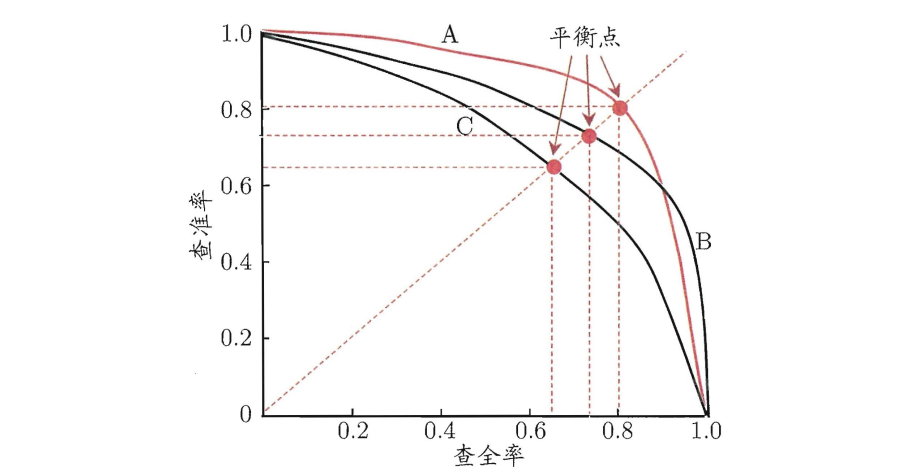
\includegraphics[width=0.8\textwidth]{../img/2-3-P-R曲线与平衡点示意图.png}
    \caption{$P-R$ 曲线与平衡点示意图}
    \label{fig: $P-R$ 曲线与平衡点示意图}
\end{figure}

$P-R$ 图直观地显示出学习器在样本总体上的查全率、查准率。在进行比较时,若一个学习器的 $P-R$ 曲线被另一个学习器的 $P-R$ 曲线完全“包住”,则可断言后者的性能优于前者。如果两个学习器的 $P-R$ 曲线发生了交叉,这时我们就需要用其他性能度量来比较学习器的性能。

“平衡点”(Break-Event Point, BEP)是“查准率 $=$ 查全率”时的取值,我们可以基于平衡点进行比较,如图中 $A$ 优于 $B$。

但是平衡点过于简化了,更常用的是 $F1$ 度量:
\begin{equation*}
    F1 = \frac{2 \times P \times R}{P + R} = \frac{2 \times TP}{\text{样例总数} + TP - TN}
\end{equation*}

在一些特定情况,我们希望对查全率或查准率有一定的偏好,可以使用 $F1$ 度量的一般形式 $F_{\beta}$:
\begin{equation*}
    F_{\beta} = \frac{(1 + \beta^2) \times P \times R}{(\beta^2 \times P) + R}
\end{equation*}

其中 $\beta > 0$ 度量了查全率对查准率的相对重要性:$\beta > 1$ 时查全率有更大影响,$\beta < 1$ 时查准率有更大影响,$\beta = 1$ 时退化为 $F1$。

注意:
\begin{enumerate}[\hspace*{2em} i.]
    \item $F1$ 是基于查准率与查全率的调和平均(harmonic mean)定义的:$\displaystyle \frac{1}{F1} = \frac{1}{2} \cdot (\frac{1}{P} + \frac{1}{R})$
    \item $F_\beta$ 是加权调和平均:$\displaystyle \frac{1}{F_\beta} = \frac{1}{1 + \beta^2} \cdot (\frac{1}{P} + \frac{\beta^2}{R})$
\end{enumerate}

很多时候我们有多个二分类混淆矩阵,例如进行多次训练(测试),每次得到一个混淆矩阵;或是在多个数据集上进行训练(测试),希望估计算法的“全局”性能;甚或是执行多酚类任务,每两两类别的组合都对应一个混淆矩阵……总之,我们希望在 $n$ 个二分类混淆矩阵上综合考察查准率和查全率。

一种直接的做法是先在各混淆矩阵上分别计算出查准率和查全率,记为:$(P_1, R_1), (P_2, R_2), \cdots, (P_n, R_n)$,再计算平均值,这样就得到“宏查准率”(macro-P)、“宏查全率”(macro-R),以及相应的“宏 $F1$”(macro-F1):
\begin{equation*}
    \text{macro-P} = \frac{1}{n} \sum_{i = 1}^{n} P_i \ \ \ \text{macro-R} = \frac{1}{n} \sum_{i = 1}^{n} R_i
\end{equation*}
\begin{equation*}
    \text{macro-F1} = \frac{2 \times \text{macro-P} \times \text{macro-R}}{\text{macro-P} + \text{macro-R}}
\end{equation*}

还可以先将各混淆矩阵的对应元素进行平均,得到 $TP, FP, TN, FN$ 的平均值,分别记为 $\overline {TP}, \overline{FP}, \overline{TN}, \overline{FN}$,再基于这些平均值计算出“微查准率”(micro-P)、“微查全率”(micro-R)和“微 $F1$”(micro-F1):
\begin{equation*}
    \text{micro-P} = \frac{\overline{TP}}{\overline{TP} + \overline{FP}} \ \ \ \text{micro-R} = \frac{\overline{TP}}{\overline{TP} + \overline{FN}}
\end{equation*}
\begin{equation*}
    \text{micro-F1} = \frac{2 \times \text{micro-P} \times \text{micro-R}}{\text{micro-P} + \text{micro-R}}
\end{equation*}

\subsection{ROC 与 AUC}

很多学习器是为测试样本产生一个实值或概率预测,然后将这个预测值与一个分类阈值(threshold)进行比较,若大于阈值则分为正类,否则为反类。实际上,根据这个实值或概率预测结果,我们可将测试样本进行排序,“最可能”是正例的排在最前面,“最不可能”是正例的排在后面。这样,分类过程就相当于在这个排序中以某个“截断点”(cur point)将样本分为两部分,前一部分为正例,后一部分为反例。

在不同的应用任务中,我们可以根据不同需求采用不同的截断点。因此,排序本身的质量好坏,体现了综合考虑学习器在不同任务下的“期望泛化性能”的好坏。$ROC$ 曲线则是从这个角度出发来研究学习器泛化性能的有力工具。

$ROC$ 全称是“受试者工作特征”(Receiver Operating Characteristic)曲线,与 $P-R$ 曲线不同,$ROC$ 曲线的纵轴是“真正例率”(True Positive Rate, TPR),横轴是“假正例率”(False Positive Rate, FPR),两个分别定义为:
\begin{equation*}
    TPR = \frac{TP}{TP + FN} \ \ \ FPR = \frac{FP}{TN + FP}
\end{equation*}

\begin{figure}[H]
    \centering
    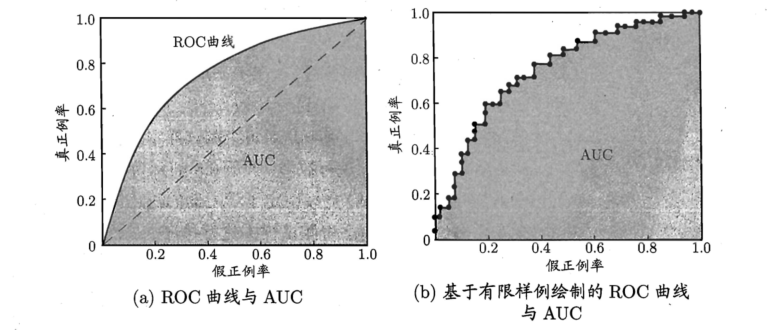
\includegraphics[width=0.8\textwidth]{../img/2-4-ROC曲线与AUC.png}
    \caption{ROC 曲线与 AUC 示意图}
    \label{fig:ROC 曲线与 AUC 示意图}
\end{figure}

现实任务中通常是利用有限个测试样例来绘制 $ROC$ 图,此时仅能获得有限个(真正利率,假正例率)坐标对。绘图过程很简单:给定 $m^+$ 个正例和 $m^-$ 个反例,根据学习器预测结果对样例进行排序,然后把分类阈值设为最大,即把所有样例均预测为反例,此时真正例率和假正例率均为 $0$,在坐标 $(0, 0)$ 处标记一个点。然后,将分类阈值依次设为每个样例的预测值,即依次将每个样例划分为正例。设前一个标记点坐标为 $(x, y)$,当前若为真正例,则对应标记点的坐标为 $\displaystyle (x, y + \frac{1}{m^+})$;当前若为假正例,则对应标记点的坐标为 $\displaystyle (x + \frac{1}{m^-}, y)$,然后用线段连接相邻点即得。

进行学习器的比较时,与 $P-R$ 图类似,若一个学习器的 $ROC$ 曲线被另一个学习器的曲线完全“包住”,则可断言后者的性能优于前者。但若两个学习器的 $ROC$ 曲线发生交叉,此时比较合理的判据是比较 $ROC$ 曲线下的面积,即 $AUC$(Area Under ROC Curve)

从定义可知,$AUC$ 可通过对 $ROC$ 曲线下各部分的面积求和而得,可估算为:
\begin{equation*}
    AUC = \frac{1}{2} \sum_{i = 1}^{m - 1} (x_{i + 1} - x_i) \cdot (y_i + y_{i + 1})
\end{equation*}

形式化地看,$AUC$ 考虑的是样本预测的排序质量,因此它与排序误差有紧密联系。给定 $m^+$ 个正例和 $m^-$ 个反例,令 $D^+$ 和 $D^-$ 分别表示正、反例集合,则排序“损失”(loss)定义为:
\begin{equation*}
    \ell_{rank} = \frac{1}{m^+ m^-} \sum_{x^+ \in D^+} \sum_{x^- \in D^-} \left(\mathbb{I} (f(x^+) < f(x^-)) + \frac{1}{2} \mathbb{I} (f(x^+) = f(x^-)) \right)
\end{equation*}

即考虑每一对正、反例,若正例的预测值小于反例,则记一个“罚分”;若相等,则记 $0.5$ 个罚分。容易看出,$\ell_{rank}$ 对应的是 $ROC$ 曲线之上的面积:若一个正例在 $ROC$ 曲线上对应标记点的坐标为 $(x, y)$,则 $x$ 恰是排序在其之前的反例所占的比例,即假正例率。因此有:
\begin{equation*}
    AUC = 1 - \ell_{rank}
\end{equation*}

\subsection{代价敏感错误率与代价曲线}

在上面的方法中,将学习器的犯错同等对待。但在现实生活中,将正例预测成假例与将假例预测成正例的代价常常是不一样的。因此,为权衡不同类型错误所造成的损失,可为错误赋予“非均等代价”(unequal cost)。

以二分类任务为例,由此引入了“代价矩阵”(cost matrix):

\begin{figure}[H]
    \centering
    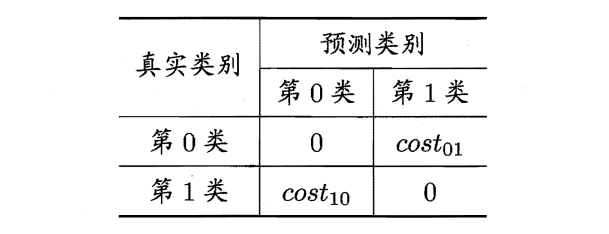
\includegraphics[width=0.8\textwidth]{../img/2-5-二分类代价矩阵.png}
    \caption{二分类代价矩阵}
    \label{fig:二分类代价矩阵}
\end{figure}

在非均等代价下,我们所希望的不再是简单地最小化错误次数,而是希望最小化“总体代价”(total cost)。这样的“代价敏感”(cost-sensitive)错误率为:
\begin{equation*}
    E(f; D; cost) = \frac{1}{m} \left(
        \sum_{x_i \in D^+} \mathbb{I} (f(x_i) \ne y_i) \times cost_{01} + \sum_{x_i \in D^-} \mathbb{I} (f(x_i) \ne y_i) \times cost_{10}
    \right)
\end{equation*}

在非均等代价下,$ROC$ 曲线不能直接反映出学习器的期望总体代价,而“代价曲线”(cost curve)则可达到该目的。代价曲线图的横轴是取值为 $[0, 1]$ 的正例概率代价:
\begin{equation*}
    P(+)cost = \frac{p \times cost_{01}}{p \times cost_{01} + (1 - p) \times cost_{10}}
\end{equation*}
其中 $p$ 是样例为正例的概率;纵轴是取值为 $[0, 1]$ 的归一化代价:
\begin{equation*}
    cost_{norm} = \frac{FNR \times p \times cost_{01} + FPR \times (1 - p) \times cost_{10}}{p \times cost_{01} + (1 - p) \times cost_{10}}
\end{equation*}

代价曲线的绘制很简单:设 $ROC$ 曲线上每一点对应了代价平面上的一条线段,设 $ROC$ 曲线上点的坐标为 $(TPR, FPR)$,则可相应计算出 $FNR$,然后再代价平面上绘制一条从 $(0, FPR)$ 到 $(1, FNR)$ 的线段,线段下的面积即表示了该条件下的期望总体代价;如此将 $ROC$ 曲线上的每个点转化为代价平面上的一条线段,然后取所有线段的下界,围成的面积即为在所有条件下学习器的期望总体代价,如下图所示:

\begin{figure}[H]
    \centering
    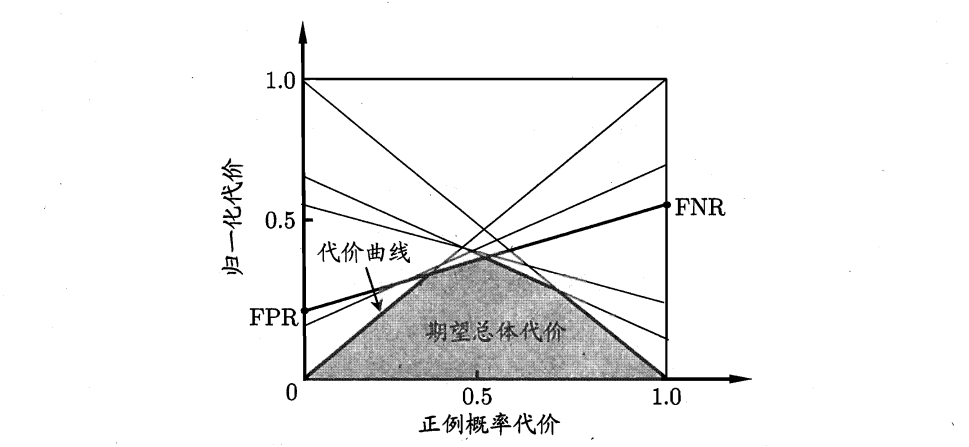
\includegraphics[width=0.9\textwidth]{../img/2-6-正例概率代价.png}
    \caption{正例概率代价}
    \label{fig:正例概率代价}
\end{figure}

\section{比较检验}

在比较学习器泛化性能的过程中,统计假设检验(hypothesis test)为学习器性能比较提供了重要依据,即若 $A$ 在某测试集上的性能优于 $B$,那 $A$ 学习器比 $B$ 好的把握有多大。

为方便论述,本篇中都以“错误率”作为性能度量的标准。

\subsection{假设检验}

假设检验中的“假设”是对学习器泛化错误率分布的某种判断或猜想,例如 $\epsilon = \epsilon_0$。现实任务中我们并不知道学习器的泛化错误率,只能获知其测试错误率 $\hat{\epsilon}$。泛化错误率与测试错误率未必相同,但直观上,二者接近的可能性应比较大,相差很远的可能性比较小。因此,可根据测试错误率估推储泛化错误率的分布。

泛化错误率为 $\epsilon$ 的学习器在一个样本上犯错的概率是 $\epsilon$;测试错误率 $\hat{\epsilon}$ 意味着在 $m$ 个测试样本中恰有 $\hat{\epsilon} \times m$ 个被误分类。假定测试样本是从样本总体分布中独立采样而得,那么泛化错误率为 $\epsilon$ 的学习器将其中 $m^\prime$ 个样本误分类、其余样本全都分类正确的概率是 $\epsilon^{m^\prime} (1 - \epsilon)^{m - m^\prime}$;由此可估算出其恰将 $\hat{\epsilon} \times m$ 个样本误分类的概率如下式所示,这也表达了在包含 $m$ 个样本的测试集上,泛化错误率为 $\epsilon$ 的学习器被测得测试错误率为 $\hat{\epsilon}$ 的概率:
\begin{equation*}
    P(\hat{\epsilon}; \epsilon) = \left( {\begin{array}{*{20}{c}}
        m\\
        {\hat{\epsilon} \times m}
        \end{array}} \right) \epsilon^{\hat{\epsilon} \times m} (1 - \epsilon) ^{m - \hat{\epsilon} \times m}
\end{equation*}

给定测试错误率,则解 $\displaystyle \frac{\partial P (\hat{\epsilon}; \epsilon)}{\partial \epsilon} = 0$ 可知,$P (\hat{\epsilon}; \epsilon)$ 在 $\epsilon = \hat{\epsilon}$ 时最大,$|\epsilon - \hat{\epsilon}|$ 增大时 $P (\hat{\epsilon}; \epsilon)$ 减小。这符合二项(binomial)分布,如下图所示,若 $\epsilon = 0.3$,则 $10$ 个样本中测得 $3$ 个被误分类的概率最大。

\begin{figure}[H]
    \centering
    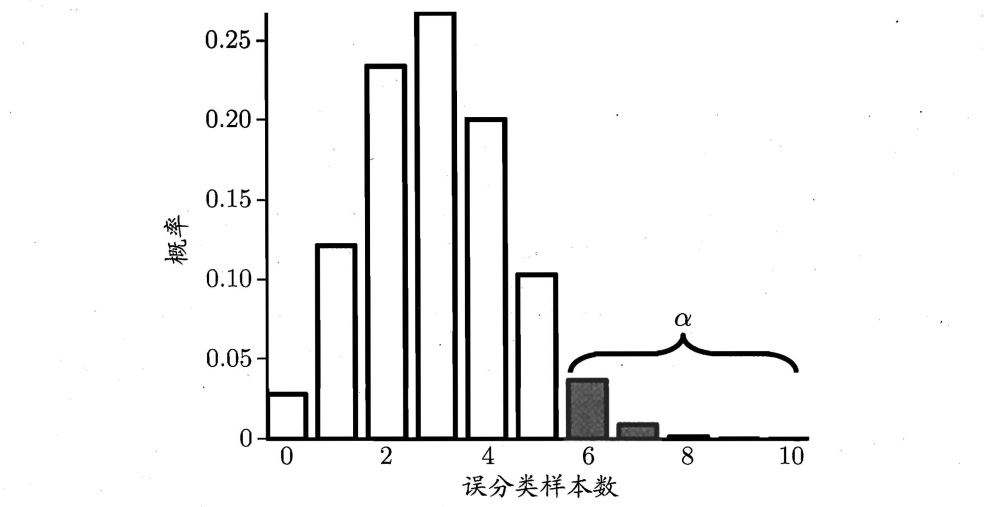
\includegraphics[width=0.8\textwidth]{../img/2-7-二项分布示意图.png}
    \caption{二项分布示意图($m = 10, \epsilon = 0.3$)}
    \label{fig:二项分布示意图}
\end{figure}

我们可以使用“二项检验”(binomial test)来对“$\epsilon \le 0.3$”(即“泛化错误率是否大不大于 $0.3$”)这样的假设进行检验。更一般的,考虑假设“$\epsilon \le \epsilon_0$,则在 $1 - \alpha$ 的概率内所能观测到的最大错误率如下式计算。这里 $1 - \alpha$ 反映了结论的“置信度”(confidence),直观地来看,相应与图 \ref{fig:二项分布示意图} 中非阴影部分的范围。
\begin{equation*}
    \bar{\epsilon} = \max \epsilon \ \ \ s.t. \ \ \sum_{i = \epsilon_0 \times m + 1}^{m} \left( {\begin{array}{*{20}{c}}
        m\\
        i
        \end{array}} \right) \epsilon^i (1 - \epsilon)^{m - i} < \alpha
\end{equation*}

此时若测试错误率 $\hat{\epsilon}$ 小于临界值 $\bar{\epsilon}$,则根据二项检验可得出结论:在 $\alpha$ 的显著度下,假设“$\epsilon \le \epsilon_0$”不能被拒绝,即能以 $1 - \alpha$ 的置信度认为,学习器的泛化错误率不大于 $\epsilon_0$;否则该假设可被拒绝,即在 $\alpha$ 的显著度下可认为学习器的泛化错误率大于 $\epsilon_0$。

注意:
\begin{enumerate}[\hspace*{2em} i.]
    \item $\alpha$ 常用取值有 $0.05, 0.1$,图 \ref{fig:二项分布示意图} 中 $\alpha$ 较大是为了绘图方便。
    \item $s.t.$ 是“subject to”的简写,使左边式子在右边条件满足时成立。
\end{enumerate}

在很多时候我们并非仅做一次留出法估计,而是通过多次重复留出法或是交叉验证法等进行多次训练(测试),这样回答得到多个测试错误率,此时可使用“$t$ 检验”($t-test$)。假定我们得到了 $k$ 个测试错误率,$\hat{\epsilon_1}, \hat{\epsilon_2}, \cdots, \hat{\epsilon_k}$,则平均测试错误率 $\mu$ 和方差 $\sigma^2$ 为:
\begin{equation*}
    \mu = \frac{1}{k} \sum_{i = 1}^{k} \hat{\epsilon_i} \ \ \ \sigma^2 = \frac{1}{k - 1} \sum_{i = 1}^{k} (\hat{\epsilon_i} - \mu)^2
\end{equation*}

考虑到这 $k$ 个测试错误率可看作泛化错误率 $\epsilon_0$ 的独立采样,则变量
\begin{equation*}
    \tau _t = \frac{\sqrt{k}(\mu - \epsilon_0)}{\sigma}
\end{equation*}
服从自由度为 $k - 1$ 的 $t$ 分布,如下图所示:

\begin{figure}[H]
    \centering
    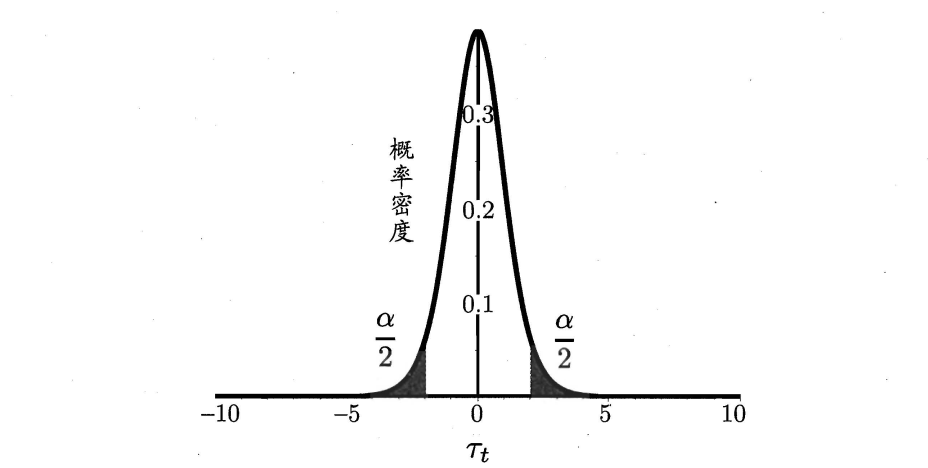
\includegraphics[width=0.8\textwidth]{../img/2-8-t分布示意图.png}
    \caption{t分布示意图($k = 10$)}
    \label{fig:t分布示意图}
\end{figure}

对假设“$\mu = \epsilon_0$”和显著度 $\alpha$,我们可以计算出当测试错误率均值为 $\epsilon_0$ 时,在 $1 - \alpha$ 概率内能观测到的最大错误率,即临界值。

这里考虑双边(two-tailed)假设,如图 \ref{fig:t分布示意图} 所示,两边阴影都各有 $\displaystyle \frac{\alpha}{2}$ 的面积;假定阴影部分范围分别为 $[-\infty, t_{- \alpha / 2}]$ 和 $[t_{\alpha / 2}, \infty]$。若平均错误率 $\mu$ 与 $\epsilon_0$ 之差 $|\mu - \epsilon_0|$ 位于临界值范围 $[t_{- \alpha / 2}, t_{\alpha / 2}]$ 内,则不能拒绝假设“$\mu = \epsilon_0$”,即可认为泛化错误率为 $\epsilon_0$,置信度为 $1 - \alpha$;否则可拒绝该假设,即在该显著度下可认为泛化错误率与 $\epsilon_0$ 有显著不同。$\alpha$ 常用取值有 $0.05, 0.1$,下图给出了一些常用临界值:

\begin{figure}[H]
    \centering
    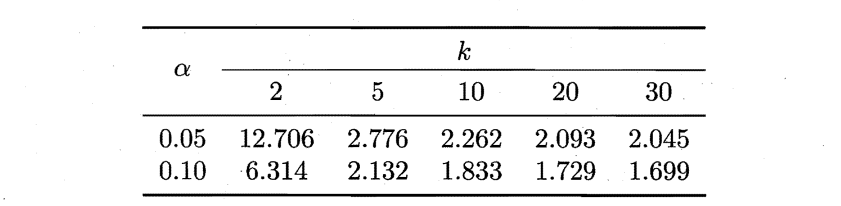
\includegraphics[width=0.8\textwidth]{../img/2-9-双边t检验的常用临界值.png}
    \caption{双边 $t$ 检验的常用临界值}
    \label{fig:双边t检验的常用临界值}
\end{figure}

上面介绍的两种方法都是对关于单个学习器泛化性能的假设进行检验,而在现实任务重,更多时候我们需要对不同学习器的性能进行比较,下面将介绍适用于此类情况的假设检验方法。

\subsection{交叉验证 t 检验}

对两个学习器 $A$ 和 $B$,若我们使用 $k$ 折交叉验证法得到的测试错误率分别为 $\epsilon_1^A, \epsilon_2^A, \cdots, \epsilon_k^A$ 和 $\epsilon_1^B, \epsilon_2^B, \cdots, \epsilon_k^B$,其中 $\epsilon_i^A$ 和 $\epsilon_i^B$ 是在相同的第 $i$ 折训练(测试)集上得到的结果,则可用 $k$ 折交叉验证“成对 $t$ 检验”(paired t-tests)来进行比较检验。这里的基本思想是若两个学习器的性能相同,则它们使用相同的训练(测试)集得到的测试错误率应相同,即 $\epsilon_i^A = \epsilon_i^B$。

具体来说,对 $k$ 折交叉验证产生的 $k$ 对测试错误率:先对每对结果求差,$\Delta_i = \epsilon_i^A - \epsilon_i^B$;若两个学习器性能相同,则差值均值应为零。因此,可根据差值 $\Delta_1, \Delta_2, \cdots, \Delta_k$ 来对“学习器 $A$ 与 $B$ 性能相同”这个假设做 $t$ 检验,计算出差值的均值 $\mu$ 和方差 $\sigma^2$,在显著度 $\alpha$ 下,若变量:
\begin{equation*}
    \tau_t = \left | \frac{\sqrt{k} \mu}{\sigma} \right | 
\end{equation*}
小于临界值 $t_{\alpha / 2, k - 1}$,则假设不能被拒绝,即认为两个学习器的性能没有显著差别;否则可认为两个学习器的性能有显著差别,且平均错误率较小的那个学习器性能较优。这里 $t_{\alpha / 2, k - 1}$ 是自由度为 $k - 1$ 的 $t$ 分布上尾部累积分布为 $\alpha / 2$ 的临界值。

欲进行有效的假设检验,一个重要前提是测试错误率均为泛化错误率的独立采样.然而,通常情况下由于样本有限,在使用交叉验证等实验估计方法时,不同轮次的训练集会有一定程度的重叠,这就使得测试错误率实际上并不独立,会导致过高估计假设成立的概率.为缓解这一问题,可采用“$5 \times 2$ 交叉验证”。

$5 \times 2$ 交叉验证是做 5 次 2 折交叉验证,在每次 2 折交叉验证之前随机将数据打乱,使得 $5$ 次支又验证中的数据划分不重复.对两个学习器 $A$ 和 $B$,第 $i$ 次 $2$ 折交叉验证将产生两对测试错误率,我们对它们分别求差,得到第 $1$ 折上的差值 $\Delta_i^1$ 和第 $2$ 折上的差值 $\Delta_i^2$。 为缓解测试错误率的非独立性,我们仅计算第 $1$ 次 $2$ 折交叉验证的两个结果的平均值 $\mu = 0.5(\Delta_1^1 + \Delta_1^2)$,但对每次 $2$ 折实验的结果都计算出其方差 $\displaystyle \sigma_i^2 = \left(\Delta_i^1 - \frac{\Delta_i^1 + \Delta_i^2}{2} \right)^2 + \left(\Delta_i^2 - \frac{\Delta_i^1 + \Delta_i^2}{2} \right)^2$。

变量:
\begin{equation*}
    \tau_t = \frac{\mu}{0.2 \sum_{i = 1}^{5} \sigma_i^2}
\end{equation*}
服从自由度为 $5$ 的 $t$ 分布,其双边检验的临界值 $t_{\alpha / 2, 5}$ 当 $\alpha = 0.05$ 时为 $2.5706$,当 $\alpha - 0.1$ 时为 $2.0150$。



\end{document}